\section{Sprint 1}
Lors du premier sprint, nous avons dû mettre en place la base du programme. Pour le modèle, il s'agissait de mettre en place les classes :
\begin{itemize}
\item Turtle qui représente une tortue, 
\item Point, pour stocker les coordonnées d'une tortue,
\item Line, qui permettent aux tortues de laisser une trace (instruction pendown)
\item World
\end{itemize}
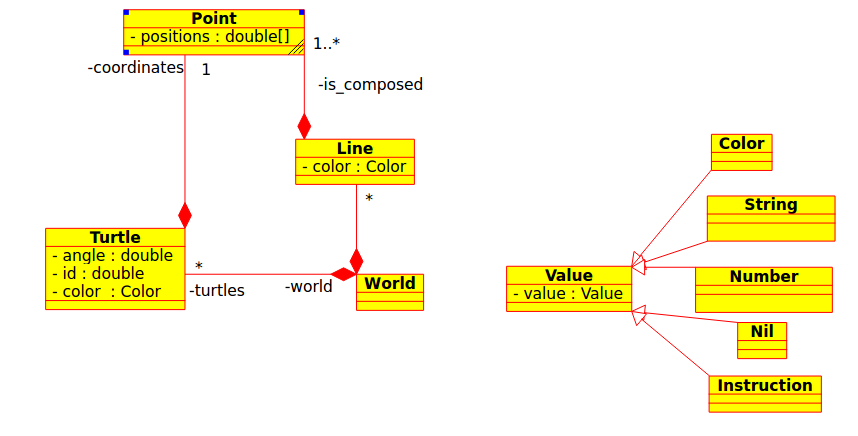
\includegraphics[scale=0.5]{doc/report/uml/v01.png}
La classe World représente le monde des tortues. Il contient la liste des tortues, et les lignes tracées par ces tortues.
Nous mettons aussi en place certains types Stibbons, comme Color, pour la couleur, ou Nil qui est une valeur nulle. Ils héritent de Value, une classe abstraite qui contient une valeur et ses accesseurs.\\

A la fin du premier sprint, nous avions réalisé ce schéma, en dehors de la classe Instruction qui n'était finalement pas nécessaire. Les instructions tel que pendown, forward, etc... sont finalement des mots clés dans la grammaire du langage.\\
CAPTURE D'ECRAN DE L'APPLI

\section{Sprint 2}
Pour le second sprint, nous avons ajouté une classe Agent, car les classes World, Turtle et Zone sont des agents, au sens multi-agent. Ils ont chacun un parent, celui qui l'a créer, une liste d'enfant, et des propriétés. Les propriétés sont des variables définit par l'utilisateur lors de la définition du code de l'agent, donc surtout utile pour les tortues.
Le monde a une taille, une liste de "breed", d'espèce. Il y a les espèces nommées et les "anonymes", qui sont des turtles dans le code.
Comme le montre ce code, on peut créer des tortues nommées ou pas.\\
METTRE UN EXEMPLE DE CODE DE L'UTILISATION DE BREED\\

Nous avons mis en place les mutexs.
Les types stibbons sont les mêmes, mais leurs définitions s'est un peu compléxifier en passant par une classe Simple-value, pour la mise en place des mutexs. Une énumeration des types Stibbons existe, elle est utiliser avec la méthode getType() pour pouvoir connaître le type de Value.\\
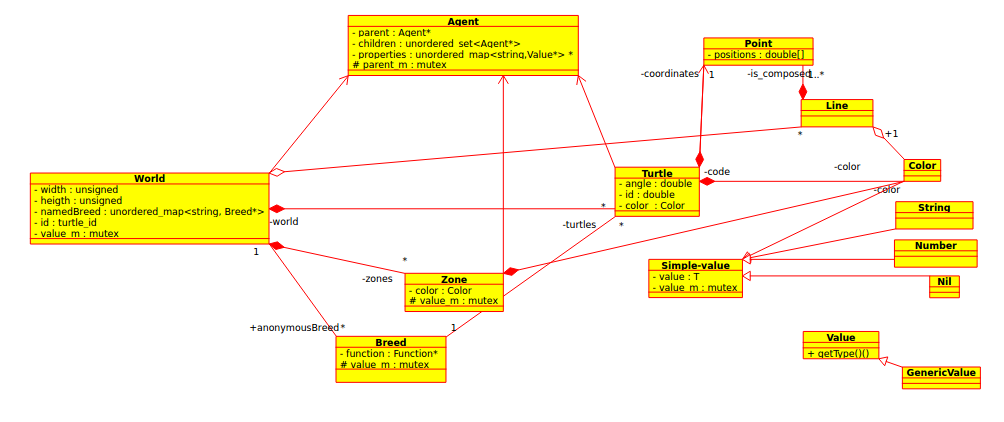
\includegraphics[scale=0.4]{doc/report/uml/v02reel.png}
CAPTURE D'ECRAN DE L'APPLI

\section{Sprint 3}


